\subsubsection{UCA 1 - Accesso all'applicazione}%kite level

\begin{figure}[h]
  \centering
    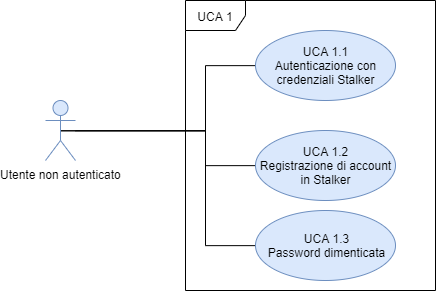
\includegraphics[scale=0.5]{sezioni/UseCase/Immagini/UCA1.png}
  \caption{UCA 1 - Accesso all'applicazione}
\end{figure}

\begin{itemize}
\item \textbf{Attori primari:} Utente non autenticato
\item \textbf{Precondizione:} L'utente non è autenticato.
\item \textbf{Postcondizione:} L'utente viene autenticato all'interno del sistema tramite registrazione [UCA 1.2] oppure tramite autenticazione\ap{G} [UCA 1.1].
\item \textbf{Scenario principale:} L'utente non identificato può scegliere se registrarsi [UCA 1.2] nel sistema oppure, se possiede già un account, accedere [UCA 1.1] all'applicazione. %cosa potrebbe fare l'utente con il UC, descrizione
\end{itemize}

\subsubsection{UCA 1.1 - Autenticazione con credenziali Stalker}%sea level

\begin{figure}[h]
  \centering
    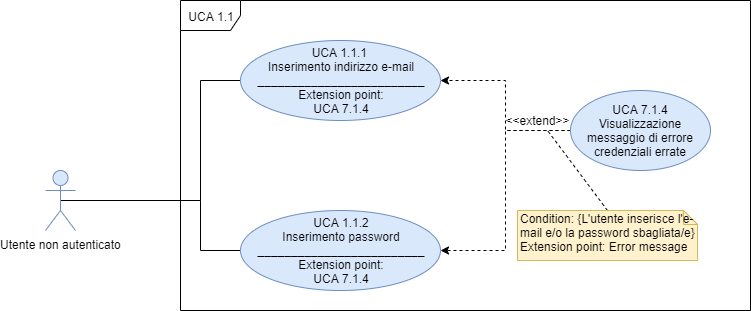
\includegraphics[scale=0.5, center]{sezioni/UseCase/Immagini/UCA1.1.png}
  \caption{UCA 1.1 - Autenticazione\ap{G} con credenziali Stalker}
\end{figure}

\begin{itemize}
\item \textbf{Attori primari:} Utente non autenticato
\item \textbf{Precondizione:} L'utente non è autenticato.
\item \textbf{Postcondizione:} L'utente viene autenticato all'interno del sistema e accede all'applicazione.
\item \textbf{Scenario principale:} L'utente non autenticato inserisce l'indirizzo e-mail e la password per autenticarsi attraverso il modulo di login\ap{G} presente.
\item \textbf{Scenario alternativo 1:} L'utente tenta di accedere con delle credenziali errate [UCS 8.1.4].
\item \textbf{Scenario alternativo 2:} Se l'utente non dovesse ricordarsi la password ha la possibilità di selezionare la funzionalità password dimenticata [UCA 1.3] per reimpostarla.
\item \textbf{Flusso di eventi:}
  \begin{enumerate}
        \item Inserimento indirizzo e-mail [UCA 1.1.1];
        \item Inserimento password [UCA 1.1.2].
    \end{enumerate}
\item \textbf{Estensioni:}
	\begin{itemize}
		\item UCA 8.1.4 - Visualizzazione messaggio di errore credenziali errate;
		\item UCA 1.3 - Password dimenticata.
	\end{itemize}
%\item \textbf{Inclusioni:}
\end{itemize}

\subsubsection{UCA 1.1.1 - Inserimento indirizzo e-mail}%fish level
\begin{itemize}
\item \textbf{Attori primari:} Utente non autenticato
\item \textbf{Precondizione:} L'utente non è autenticato.
\item \textbf{Postcondizione:} L'utente ha inserito il proprio indirizzo e-mail.
\end{itemize}

\subsubsection{UCA 1.1.2 - Inserimento password}%fish level
\begin{itemize}
\item \textbf{Attori primari:} Utente non autenticato
\item \textbf{Precondizione:} L'utente non è autenticato.
\item \textbf{Postcondizione:} L'utente ha inserito la propria password.
\end{itemize}

\subsubsection{UCA 1.2 - Registrazione di account in Stalker}%sea level

\begin{figure}[h]
  \centering
    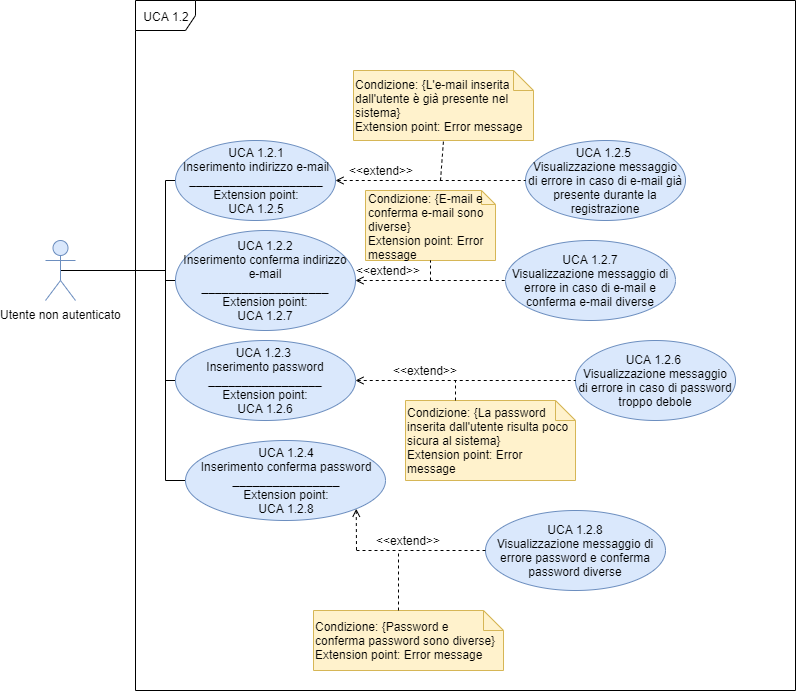
\includegraphics[scale=0.4, center]{sezioni/UseCase/Immagini/UCA1.2.png}
  \caption{UCA 1.2 -  Registrazione di account in Stalker}
\end{figure}

\begin{itemize}
\item \textbf{Attori primari:} Utente non autenticato
\item \textbf{Precondizione:} L'utente non è ancora registrato nel sistema.
\item \textbf{Postcondizione:} L'utente si è registrato e accede al sistema.
\item \textbf{Scenario principale:} L'utente non registrato compila il modulo di registrazione al fine di poter accedere al sistema.
\item \textbf{Flusso di eventi:}
  \begin{enumerate}
        \item Inserimento indirizzo e-mail [UCA 1.2.1];
        \item Inserimento password [UCA 1.2.2];
        \item Inserimento conferma password [UCA 1.2.3];
        \item Accettazione delle condizioni generali d'uso [UCA 1.2.4];
    \end{enumerate}
\end{itemize}

\subsubsection{UC 1.2.1 - Inserimento indirizzo e-mail}%fish level

\begin{itemize}
\item \textbf{Attori primari:} Utente non autenticato
\item \textbf{Precondizione:} L'utente non è registrato.
\item \textbf{Postcondizione:} L'utente ha inserito il proprio indirizzo e-mail, di cui è stata verificata la non esistenza in associazione ad altri account nel sistema.
\item \textbf{Estensioni:}
	\begin{itemize}
		\item UCA 8.1.1 - Visualizzazione messaggio di errore in caso di account con l'e-mail inserita già presente.
	\end{itemize}
\end{itemize}

\subsubsection{UCA 1.2.2 - Inserimento password}%fish level
\begin{itemize}
\item \textbf{Attori primari:} Utente non autenticato
\item \textbf{Precondizione:} L'utente non è registrato.
\item \textbf{Postcondizione:} L'utente ha inserito una password che rispetta i criteri di complessità definiti dal sistema.
\item \textbf{Estensioni:}
	\begin{itemize}
		\item UCA 8.1.2 - Visualizzazione messaggio di errore in caso di password troppo debole.
	\end{itemize}
\end{itemize}

\subsubsection{UCA 1.2.3 - Inserimento conferma password}%fish level
\begin{itemize}
\item \textbf{Attori primari:} Utente non autenticato
\item \textbf{Precondizione:} L'utente non è registrato.
\item \textbf{Postcondizione:} L'utente ha confermato la password inserendola nuovamente (è uguale a quella inserita durante l'inserimento della password [UCA 1.2.2]).
\item \textbf{Estensioni:}
	\begin{itemize}
		\item UCA 8.1.3 - Visualizzazione messaggio di errore in caso di password e conferma password diverse.
	\end{itemize}
\end{itemize}

\subsubsection{UCA 1.2.4 - Accettazione delle condizioni generali d'uso}%fish level
\begin{itemize}
\item \textbf{Attori primari:} Utente non autenticato
\item \textbf{Precondizione:} L'utente non è registrato.
\item \textbf{Postcondizione:} L'utente ha accettato le condizioni generali sull'uso.
\item \textbf{Scenario alternativo:} Se l'utente dovesse rifiutare le condizioni generali sull'uso allora la registrazione verrebbe interrotta e l'applicazione chiusa.
\end{itemize}

\subsubsection{UCA 1.3 - Password dimenticata}%fish level
\begin{itemize}
\item \textbf{Attori primari:} Utente non autenticato
\item \textbf{Precondizione:}  L'utente non è autenticato.
\item \textbf{Postcondizione:} L'utente ha fatto richiesta per avviare la procedura di password dimenticata.
\item \textbf{Flusso di eventi:}
  \begin{enumerate}
        \item Inserimento dell'indirizzo e-mail a cui inviare la e-mail per il cambio password [UCA 1.3.1];
        \item Viene inviata la e-mail per il cambio password [UCA 1.3.2];
        \item Inserimento della nuova password [UCA 1.3.3];
        \item Inserimento della conferma della nuova password [UCA 1.3.4].
    \end{enumerate}
\end{itemize}

\subsubsection{UCA 1.3.1 - Inserimento e-mail}
\begin{itemize}
\item \textbf{Attori primari:} Utente non autenticato
\item \textbf{Precondizione:} L'utente non è autenticato.
\item \textbf{Postcondizione:} L'utente ha inserito l'e-mail.
\end{itemize}

\subsubsection{UCA 1.3.2 - E-mail cambio password}
\begin{itemize}
\item \textbf{Attori primari:} Utente non autenticato
\item \textbf{Precondizione:} L'utente non è autenticato.
\item \textbf{Postcondizione:} L'utente riceve l'email per il cambio password, ne consegue la necessità di reimpostare la password [UCS 1.3.3 e UCS 1.3.4].
\end{itemize}

\subsubsection{UCA 1.3.3 - Nuova password}
\begin{itemize}
\item \textbf{Attori primari:} Utente non autenticato
\item \textbf{Precondizione:}  L'utente non è autenticato.
\item \textbf{Postcondizione:} L'utente inserisce la nuova password.
\end{itemize}

\subsubsection{UCA 1.3.4 - Conferma nuova password}
\begin{itemize}
\item \textbf{Attori primari:} Utente non autenticato
\item \textbf{Precondizione:} L'utente non è autenticato.
\item \textbf{Postcondizione:} L'utente reinserisce la nuova password per confermarla.
\end{itemize}

% \subsubsection{UCA 1.3.5 - Conferma cambio password}%fish level
% \begin{itemize}
% \item \textbf{Attori primari:} Utente non autenticato\ap{G}
% \item \textbf{Precondizione:} L'utente non è autenticato\ap{G}.
% \item \textbf{Postcondizione:} L'utente ha selezionato la funzionalità di conferma per il cambio password.
% \end{itemize}